
%\part{安全}


%\section{安全概述}

% \begin{frame}{安全策略}
%	\tableofcontents[currentsection]
%
%%
%%目标
%%\begin{itemize}
%%\item 理解系统性能安全目标
%%\item 解释维护系统状态的好处
%%\item 描述网络资源
%%\item 描述数据存储资源
%%\item 描述进程资源
%%\item 描述日志分析
%%\end{itemize}
%
%\end{frame} 

%\subsection{安全原则}
%
%
% \begin{frame}{安全原则}
%\begin{itemize}
%\item 物理安全
%\item 本地安全
%\item 远程安全
%\item 个人安全
%\end{itemize}
%
%\end{frame} 
%\begin{frame}{安全实践}
%\begin{itemize}
%\item 经过设计,系统通过有效的资源服务
%\item 根据策略,系统保护有效的资源
%\item 主机应该仅提供必须的服务,以及提供那些必须的人
%
%\begin{itemize}
%\item 我需要或者知道主机提供了什么吗?
%\item 他们需要或者知道访问这些服务吗?
%\item 系统行为和记录一致吗?
%\item 应用了所有相关安全补丁吗?
%\end{itemize}
%\item 监控系统资源,了解系统性能以及漏洞
%\end{itemize}
%
%\end{frame} 
%
%
% \begin{frame}{安全策略:人}
%\begin{itemize}
%\item 管理人的活动
%\item 谁管理什么
%\item 谁能对虚假警报做最终决定
%\item 什么时候可以通知执法机关
%\end{itemize}
%
%\end{frame} 
%
%
% \begin{frame}{安全策略:系统}
%\begin{itemize}
%\item 管理系统活动
%\item 常规系统监控
%
%\begin{itemize}
%\item 日志记录到一台外部服务器,以防出现意外
%\item 使用logwatch 监控日志
%\item 监控网络带宽的出站和进站使用情况
%\end{itemize}
%\item 系统数据常规备份
%\end{itemize}
%
%\end{frame} 
%
%
% \begin{frame}{应答策略}
%\begin{itemize}
%\item 假定可疑系统是不值得信任的
%
%\begin{itemize}
%\item 不要从可疑系统上运行程序
%\item 从可信赖介质启动,校验问题
%\item 分析远程日志服务器记录的日志以及“本地”日志
%\item 从RPM数据库的只读备份里检查文件完善性
%\end{itemize}
%\item 对当前机器做一个镜像,以便将来继续分析或者搜索证据
%\item 清除系统,重新安装,如何从备份中恢复你需要的数据
%\end{itemize}
%\end{frame} 

\section{系统安全}
\begin{frame}{系统安全}
\tableofcontents[currentsection]
\end{frame}
 
 \subsection{系统监控}

\begin{frame}{系统监控的好处}
\begin{itemize}
\item 通过常规监控,系统虚拟和安全得以维护
\item 系统监控包括

\begin{itemize}
\item 网络监控和分析
\item 文件系统监控
\item 进程监控
\item 日志文件分析
\end{itemize}
\end{itemize}

\end{frame} 

 \begin{frame}{网络监控工具}
\begin{itemize}
	\item 网络接口(ip)
	
	\begin{itemize}
		\item 显示系统上有效的网络接口
	\end{itemize}
	\item 端口扫描(nmap)
	
	\begin{itemize}
		\item 显示系统提供了哪些有效服务
	\end{itemize}
	\item 包嗅探(tcpdump,wireshark)
	
	\begin{itemize}
		\item 保存和分析所有网络通信到'嗅探'系统上
	\end{itemize}
\end{itemize}

\end{frame} 

\begin{frame}{查看本地网络}
\begin{itemize}
\item ip 工具

\begin{itemize}
\item 初始化脚本调用
\item 比ifconfig功能更强
\end{itemize}
\item netstat -ntaupe 列出

\begin{itemize}
\item 活动的网络服务
\item 已建立的连接
\end{itemize}
\end{itemize}

\end{frame} 

\begin{frame}{查看远程网络}
\begin{itemize}
\item nmap 报告开放端口上的服务

\begin{itemize}
\item 有效的高级扫描选项
\item 提供远程OS探测(-O)
\item 大小子网均可扫描
\end{itemize}
\item 管理员权限下使用
\item 图形化前端程序可用(zenmap\footnote{\href{http://nmap.org/zenmap/}{http://nmap.org/zenmap}}/nmapsi4\footnote{\href{http://nmapsi4.netsons.org/web/}{http://nmapsi4.netsons.org/web/}})
\end{itemize}

\end{frame} 


 \begin{frame}{文件系统分析}
\begin{itemize}
\item 常规文件系统监控可以防止

\begin{itemize}
\item 系统资源耗尽
\item 因为缺乏访问控制而导致的系统突破点
\end{itemize}
\item 文件系统监控应该包括

\begin{itemize}
\item 数据完整性扫描
\item 可疑文件调查
\end{itemize}
\item 工具

\begin{itemize}
\item df,du
\end{itemize}
\end{itemize}

\end{frame} 


 \begin{frame}{典型的有问题的许可}
\begin{itemize}
\item 未知属主的文件可能表明系统遇到非授权访问

\begin{itemize}
\item 查看没有用户或者组的文件\\
find / -nouser -o -nogroup 
\end{itemize}
\item 文件/目录对任何人有写(o+w)许可,表示可能有问题

\begin{itemize}
\item 定位这些文件\\
find / -type f -perm -002
\item 定位这些目录\\
find / -type d -perm -002
\end{itemize}
\end{itemize}

\end{frame} 


 \begin{frame}{监控进程}
\begin{itemize}
\item 监控进程来决定

\begin{itemize}
\item 性能降低的原因
\item 可疑进程是否存在
\end{itemize}
\item 监控工具

\begin{itemize}
\item top
\item gnome-system-monitor
\item sar,rfsar
\end{itemize}
\end{itemize}

\end{frame} 
 \begin{frame}{进程监控工具}
\begin{itemize}
\item top

\begin{itemize}
\item 实时查看活动进程
\item 交互模式下杀死进程或者调整进程优先级(renice)
\item 观察系统统计数据的更新
\end{itemize}
\item GUI 监控工具

\begin{itemize}
\item gnome-system-monitor: 进程,CPU,内存监控
\item kpm: top的KDE版
\item rfsar: sar的图形化实现
\end{itemize}
\end{itemize}

\end{frame} 

% \begin{frame}{系统活动报告}
%\begin{itemize}
%\item 频繁报告
%
%\begin{itemize}
%\item cron spawns sa1,sa2
%\item sar 读取日志,生成人可读的日志
%\end{itemize}
%\item 通常用户性能调试
%
%\begin{itemize}
%\item 更多精确的统计
%
%\begin{itemize}
%\item 二进制数据库收集方法
%\item 正常时间间隔
%\end{itemize}
%\end{itemize}
%\end{itemize}
%
%\end{frame} 

% \begin{frame}{通过帐号管理进程}
%\begin{itemize}
%\item 使用PAM来控制某一个帐号的资源限制
%
%\begin{description}
%\item [{pam\_access.so}] 可以通过帐号和位置来限制访问
%\item [{pam\_time.so}] 通过日期和时间显示访问
%\item [{pam\_limits.so}] 可以限制某一个进程的有效资源
%\end{description}
%\end{itemize}
%
%\end{frame} 
% \begin{frame}{系统日志文件}
%\begin{itemize}
%\item 为什么要监控日志文件
%\item 哪些日志需要监控
%\item 日志服务
%
%\begin{itemize}
%\item 大部分守护进程发送消息到syslogd
%\item 内核消息由klogd处理
%\end{itemize}
%\end{itemize}
%
%\end{frame} 
% \begin{frame}{syslogd/klogd 配置}
%\begin{itemize}
%\item 配置文件 /etc/syslog.conf
%\item 语法:\\
%\emph{facility.priority log\_location}
%\item 实例\\
%mail.info /dev/tty8
%\end{itemize}
%
%\end{frame} 


% \begin{frame}{日志文件分析}
%\begin{itemize}
%\item 对常规部分进行分析
%\item logwatch 可以通过cron来运行,每小时来报告可能的问题
%\item 当查找反常信息时,logwatch 使用negative lists
%
%\begin{itemize}
%\item 丢失所有正常的信息
%\item 分析剩余的
%\end{itemize}
%\end{itemize}
%
%
%\end{frame} 

%\section{帐号安全管理}

%
%%
%% \begin{frame}{帐号安全管理}
%%目标
%%\begin{itemize}
%%\item 理解基本认证
%%\item 掌握sudo的配置
%%\item 理解NSS和PAM的角色
%%\end{itemize}
%%\end{frame} 
%
%
% \subsection{帐号概述}
%
%
%
% \begin{frame}{用户帐号}
%\begin{itemize}
%\item 对每一个用户帐号而言必须提供两类信息
%
%\begin{itemize}
%\item 帐号信息
%
%\begin{itemize}
%\item UID,缺省shell,家目录,组成员等
%\end{itemize}
%\item 认证
%
%\begin{itemize}
%\item 登录时,如何告知提供给登录的密码是正确的实现方法
%\end{itemize}
%\end{itemize}
%\end{itemize}
%\end{frame} 
%
%\begin{frame}{帐号信息(名称服务器)}
%\begin{itemize}
%\item 名称服务器通过访问库函数来映射名字到账户信息
%\item 最初,名称服务器仅由本地文件,比如/etc/passwd,来提供
%\item 后来通过重写libc增加了新的成名服务器,比如NIS的支持
%\end{itemize}
%
%\end{frame} 
% \begin{frame}{名称服务器交换(NSS)}
%\begin{itemize}
%\item NSS可以在不重写libc的情况下增加新的名称服务器
%
%\begin{itemize}
%\item 使用/lib/libnss\_service.so 文件
%\end{itemize}
%\item /etc/nsswitch.conf 控制以名称服务器以什么顺序来检查
%
%\begin{itemize}
%\item passwd: files nis ldap
%\end{itemize}
%\end{itemize}
%
%\end{frame} 
%
%%\begin{frame}{getent}
%%\begin{itemize}
%%\item getent \textit{database}
%%
%%\begin{itemize}
%%\item 列出指定数据库存储的所有对象
%%\item getent \textit{services}
%%\end{itemize}
%%\item getent \textit{database name}
%%
%%\begin{itemize}
%%\item 在指定数据里,查询指定名字的信息
%%\item getent passwd wgzhao
%%\end{itemize}
%%\end{itemize}
%%
%%\end{frame} 
%
%\begin{frame}{认证}
%\begin{itemize}
%\item 应用程序认证密码的传统做法是通过libc函数
%
%\begin{itemize}
%\item 对登录是提供的密码进行哈希
%\item 在NSS比较哈希后的密码
%\item 如果匹配,认证通过
%\end{itemize}
%\item 一旦认证方法改动,应用程序必须重写
%\end{itemize}
%\end{frame} 
%
% \subsection{sudo}
%
% \begin{frame}{sudo}
%\begin{itemize}
%\item 在/etc/sudoers文件里包含的账户,执行指令时:
%
%\begin{itemize}
%\item euid为0,而不是uid
%\item gid是root组的id,而不是私有组的id
%\end{itemize}
%\item 非/etc/sudoers里包含的账户企图执行sudo指令时,会通知要求和管理员(root)联系
%\item url:{} \href{http://blog.wgzhao.com/2009/03/13/using-sudo-effectively.html}{如何用好sudo}
%\end{itemize}
%\end{frame} 


%\subsection{PAM概述}
%
%
%
% \begin{frame}{Pluggable Authentication Modules(PAM)}
%\begin{itemize}
%\item Pluggable Authentication Modules 可植入认证模块
%\item 应用程序调用libpam函数认证和授权用户
%\item libpam复杂检查应用程序的PAM配置文件
%
%\begin{itemize}
%\item 可能会包括NSS检查
%\end{itemize}
%\item 共享的,动态配置代码
%\item 文档: /usr/share/doc/pam-<version>/
%\end{itemize}
%
%\end{frame} 
% \begin{frame}{PAM 操作}
%\begin{itemize}
%\item /lib/security/ PAM 模块
%
%\begin{itemize}
%\item 每一个模块执行一个测试,通过或者失败
%\item /etc/security/ 下的文件可能一些模块应该如何执行测试
%\end{itemize}
%\item /etc/pam.d/ PAM配置文件
%
%\begin{itemize}
%\item 这些文件决定如何以及何时模块被特定应用程序使用
%\end{itemize}
%\end{itemize}
%\end{frame} 
%
% \subsection{PAM配置}
%
%
%
% \begin{frame}{/etc/pam.d/ 文件: 测试}
%\begin{itemize}
%\item 测试组织成下面四个组:
%
%\begin{description}
%\item [{auth}] 认证这个用户就是那个用户
%\item [{account}] 授权帐号可以使用什么
%\item [{password}] 控制密码改变
%\item [{session}] 打开,关闭,记录会话
%\end{description}
%\item 每一个组根据需要被调用,并提供单独的结果给服务器
%\end{itemize}
%
%\end{frame} 
%
% \begin{frame}[shrink]{/etc/pam.d/ 文件:控制值}
%\begin{itemize}
%\item 控制值(Control values)决定每一个测试结果如何影响整个组的总结果
%
%\begin{description}
%\item [{required}] 模块检查必须成功,验证过程才能继续。如果当前模块检查失败,则只有当使用相同模块接口的所有模块都检查之后,当前模块的检查结果才会通知用户; 
%\item 
%\item [{requisite}] 模块检查必须成功,验证过程才能继续。不过,如果当前模块检查失败,会立即通知用户,并且返回一条第一个required或者requisite模块检查失败时输出的错误信息; 
%\item [{sufficient}] 如果模块检查失败,则这个结果会被忽略。不过,如果当前模块检查成功,同时之前没有其它的sufficient模块检查失败,则验证过程不会继续检查其它模块,用户通过验证; 
%\item [{optional}] 模块检查返回的结果被忽略。optional的模块只有在整个验证过程中没有其它的模块使用这个模块所引用的接口时才会对验证结果起作用。 
%\end{description}
%\end{itemize}
%
%\end{frame} 
% 
% \begin{frame}[fragile]{实例 /etc/pam.d/login 文件}
%
%\verbatiminput{/etc/pam.d/login}
%
%\end{frame} 
%
%\begin{frame}{system-auth 文件}
%\begin{itemize}
%	\item system-auth被广泛使用
%	\item 通过include 控制标志来调用,并不是作为一个模块(比如pam\_stack.so)
%	\item 包含标准认证测试
%	\item 可以共享给系统上的许多应用程序
%	\item 使得系统标准认证管理简单且一致
%\end{itemize}
%\end{frame}
%
% \begin{frame}{pam\_unix.so}
%\begin{itemize}
%\item 针对基于NSS的认证模块
%
%\begin{description}
%\item [{auth}] 从NSS获得哈希密码并和输入的密码哈希后进行比较
%\item [{account}] 检查密码过期
%\item [{password}] 处理本地文件或者NIS密码更改
%\item [{session}] 记录登入和登出到日志
%\end{description}
%\end{itemize}
%
%\end{frame} 
% \begin{frame}{网络认证}
%\begin{itemize}
%\item 集中密码管理
%
%\begin{description}
%\item [{pam\_krb5.so}] Kerberos 第五版许可证
%\item [{pam\_ldap.so}] LDAP 绑定
%\item [{pam\_smb\_auth.so}] 老的SMB认证
%\item [{pam\_winbind.so}] SMB,通过winbindd
%\end{description}
%\item 有些服务使用NSS/pam\_unix.so
%\end{itemize}
%\end{frame} 
%
%\begin{frame}{auth 模块}
%\begin{itemize}
%\item pam\_securetty.so 如果root帐号从没列在/etc/securetty里的终端登录,则认证失败
%\item pam\_nologin.so 如果用户不是root且文件/etc/nologin存在,则认证失败
%\item pam\_listfile.so 依据某一个文件内容列表来做认证字符检查
%
%\begin{itemize}
%\item 列出帐号可以允许或者拒绝
%\end{itemize}
%\end{itemize}
%
%\end{frame} 
% \begin{frame}{密码安全}
%\begin{itemize}
%\item pam\_unix.so MD5 密码哈希
%
%\begin{itemize}
%\item 密码哈希,难于破解
%\end{itemize}
%\item pam\_unix.so 影子密码
%
%\begin{itemize}
%\item 密码哈希,仅对root可见
%\item 设置密码有效期限
%\end{itemize}
%\item 其他模块可能支持密码老化机制
%\end{itemize}
%\end{frame} 
%
% \subsection{密码策略}
%
%
%
% \begin{frame}{密码策略}
%\begin{itemize}
%\item 密码历史
%
%\begin{itemize}
%\item pam\_unix.so 使用remember=\emph{N} 参数
%\end{itemize}
%\item 密码强度
%
%\begin{itemize}
%\item pam\_cracklib.so
%\item pam\_passwdqc.so
%\end{itemize}
%\item 登录失败监控
%
%\begin{itemize}
%\item pam\_tally.so
%\end{itemize}
%\end{itemize}
%
%\end{frame} 
% \begin{frame}{session 模块}
%\begin{itemize}
%\item pam\_limits.so 强制资源限制
%
%\begin{itemize}
%\item 使用/etc/security/limits.conf
%\end{itemize}
%\item pam\_console.so 对终端用户,设置本地设备许可
%\item pam\_selinux.so 帮助设置SELinux上下文
%\item pam\_mkhomedir.so 创建家目录,如果不存在的话
%\end{itemize}
%
%\end{frame} 
% \begin{frame}{使用工具和认证}
%\begin{itemize}
%\item 本地需要认证的管理工具
%
%\begin{itemize}
%\item su,reboot,rf{*},\ldots{}
%\end{itemize}
%\item pam\_rootok.so 如果以root运行,则通过
%\item pam\_timestamp.so 针对类似sudo行为
%\item pam\_xauth.so 转发xauth cookies
%\end{itemize}
%
%\end{frame} 
% \begin{frame}{PAM故障排除}
%\begin{itemize}
%\item 检查系统日志
%
%\begin{itemize}
%\item /var/log/messages
%\item /var/log/secure
%\end{itemize}
%\item PAM的错误可能会导致root无法登录
%
%\begin{itemize}
%\item 测试PAM时,保留一个root登录的窗口
%\item 单用户模式可以绕过PAM
%\item 系统救援模式启动系统
%\end{itemize}
%\end{itemize}
%\end{frame} 

\section{网络安全}

\begin{frame}{网络安全}

%目标
%\begin{itemize}
%%\item 理解tcp\_wrappers
%%\item 使用libwrap.so识别应用程序
%\item 理解iptables 防火墙
%\item 定制iptables防火墙规则
%\end{itemize}
\tableofcontents[currentsection]
\end{frame} 

%\subsection{tcp\_wrappers}
%\begin{comment}
%象Telnet、SSH、FTP、POP和SMTP等很多网络服务都会用到TCP Wrapper,它被设计为一个介于外来服务请求和系统服务回应的中间处理软件。 
%它的基本过程是这样的:当系统接收到一个外来服务请求的时候,先由TCP Wrapper处理这个请求,TCP Wrapper根据这个请求所请求的服务和针对这个服务所定制的存取控制规则来判断对方是否有使用这个服务的权限,如果有,TCP Wrapper将该请求按照配置文件定义的规则转交给相应的守护进程去处理同时记录这个请求动作,然后自己就等待下一个请求的处理。
% TCP Wrapper机制的主要目的在于,来自客户端的请求只被允许同一个独立的守护进程(xinetd)直接通信,而它请求的目标服务被TCP Wrapper包裹起来,这样就提高了系统的安全性和系统管理的方便性。 
%TCP Wrapper 提高了系统的安全性。系统安全性的具体体现主要有两点,一个是获取访问权限前的控制,一个是获取访问后的处理。获取权限前,它会根据/etc/hosts.allow和/etc/hosts.deny定制的规则来判断对方是否有权限;获取权限后,通过bind、redirect等属性的设置,可能已经由另一台主机或者另一个服务在处理了对方的请求,而对方并不会感知中间经过了这样的处理。 
%TCP Wrapper更加方便了系统管理。一方面可以抽取系统所有服务共有的属性放到/etc/xinetd.conf中,另一方面,将每一个服务具体的配置放到/etc/inetd.d目录下,而每个配置文件都遵循同样的语法和规则。  
%TCP Wrapper的功能来自于libwrap.a,它是一个网络服务库,象xinetd、sshd和portmap等许多系统服务编译时都依赖于它,其他的网路服务程序甚至你自己编写的网络服务程序都可以加上这个编译选项来提供TCP Wrapper的功能。
%\end{comment}
%
%\begin{frame}{tcp\_wrappers 配置}
%\begin{itemize}
%\item 访问检查的三个阶段
%
%\begin{itemize}
%\item 访问是否被明确许可
%\item 否则,访问是否被明确拒绝
%\item 如果都没有,默认许可
%\end{itemize}
%\item 配置存储在两个文件里
%
%\begin{itemize}
%\item 许可用: /etc/hosts.allow
%\item 拒绝用: /etc/hosts.deny
%\end{itemize}
%\item 基本语法
%
%\begin{itemize}
%\item \emph{守护进程列表:客户端列表 {[} :参数 {]}}
%\end{itemize}
%\end{itemize}
%
%\end{frame} 
%
%\mode<handout>
%{
%the first fields specifies a comma-delimited list of daemons.tcp_wrappers usually takes argv[0] (process name without path)as the deamon name
%example
%in.telnetd: 192.168.0.1
%sshd,gdm: 192.168.0.1
%if your host has more than one network interface and you want to implement different policies for them,use the following syntax:
%in.telnetd@192.168.0.254: 192.168.0.
%in.telnetd@192.168.1.254: 192.168.1.
%}
%
%\begin{frame}{守护进程列表}
%
%\begin{itemize}
%\item 守护进程列表应该是
%
%\begin{itemize}
%\item 服务的可执行程序名
%\item 允许指定多个服务
%\item 使用ALL 匹配所有服务
%\item 允许可执行程序名后添加IP或主机名,如果本机有多个网络接口
%\end{itemize}
%\item 高级语法
%
%\begin{itemize}
%\item \emph{deamon@host: client\_list \ldots{}}
%\end{itemize}
%\end{itemize}
%
%\end{frame} 
% \begin{frame}{客户端列表}
%
%
%\begin{itemize}
%\item 主机规范
%
%\begin{itemize}
%\item IP地址(192.168.1.1,10.0.0.)
%\item 域名或主机名(www.redflag-linux.com, .wgzhao.com)
%\item 子网掩码(192.168.1.0/255.255.255.0)
%\item 网络名(@mydomain)
%\end{itemize}
%\end{itemize}
%
%\end{frame} 
% \begin{frame}{高级客户端语法}
%\begin{itemize}
%\item 通配符
%
%\begin{itemize}
%\item ALL : 总是匹配
%\item LOCAL:所有名字不包含'.'的主机
%\item KNOWN:可以双向解析的主机或用户
%\item UNKNOWN: 无法被解析的主机或用户
%\item PARANOID:正向解析和反向解析不匹配的主机
%\end{itemize}
%\item EXCEPT
%\mode<handout>
%{
%/etc/hosts.allow
%sshd: ALL EXCEPT .cracker.org EXCEPT trusted.cracker.org
%/etc/hosts.deny
%sshd: ALL
%}
%\begin{itemize}
%\item 可以用于客户端和服务端列表
%\item 可以嵌套使用
%\end{itemize}
%\end{itemize}
%
%\end{frame} 
%
% \begin{frame}{扩充选项}
%\begin{itemize}
%\item 语法\\
%\textit{daemon\_list: client\_list {[} :opt1 :opt2 \ldots{}{]}}
%\item spwan
%
%\begin{itemize}
%\item 用来启动额外程序
%\item 特殊扩展有效(\%c,\%s)
%\end{itemize}
%\item 举例\\
%in.telnetd: ALL : spawn echo `login attempt from \%c to \%s' | mail -s warning root
%\item DENY
%
%\begin{itemize}
%\item 作为可选现用在hosts.allow 里
%\end{itemize}
%\item 举例
%
%\begin{itemize}
%\item ALL: ALL: DENY
%\end{itemize}
%\end{itemize}
%
%\end{frame} 
% \begin{frame}{tcp\_wrappers 例子}
%
%\# /etc/hosts.allow
%
%vsftpd : 192.168.1.
%
%in.telnetd,sshd : .xplore.cn 192.168.2.240
%
%\medskip{}
%
%
%\# /etc/hosts.deny
%
%ALL : ALL
%
%
%\end{frame} 
% \begin{frame}{xinetd和tcp\_wrappers}
%\begin{itemize}
%\item xinetd 提供了自己的一套访问控制
%
%\begin{itemize}
%\item 基于主机
%\item 基于时间
%\end{itemize}
%\item 在xinetd与tcp\_wrapper都限制的情况下
%
%\begin{itemize}
%\item 先检查tcp\_wrapper
%\item 如果tcp\_wrapper允许连接,再检查xinetd是否也允许
%\end{itemize}
%\end{itemize}
%\end{frame} 

\subsection{防火墙}

\begin{frame}{Netfilter 概述}
\begin{itemize}
\item 在内核中过滤,没有守护进程
\item 在OSI参考模型的2,3,4层申明
\item 仅检查包头信息
\item 由内核模块netfilter和用户空间的iptables指令组成
\end{itemize}

\end{frame} 
 \begin{frame}{Netfilter表和链}

\begin{center}
\begin{tabular}{|c|c|c|c|}
\hline 
过滤点(chain) & \multicolumn{3}{c|}{表}\tabularnewline
\cline{2-4} 
 & filter & NAT & mangle\tabularnewline
\hline 
INPUT & X &  & X\tabularnewline
\hline 
FORWARD & X &  & X\tabularnewline
\hline 
OUTPUT & X & X & X\tabularnewline
\hline 
PREROUTING &  & X & X\tabularnewline
\hline 
POSTROUTING &  & X & X\tabularnewline
\hline 
\end{tabular}
\par\end{center}


\end{frame} 
 \begin{frame}{Netfilter 包流程图}
\center
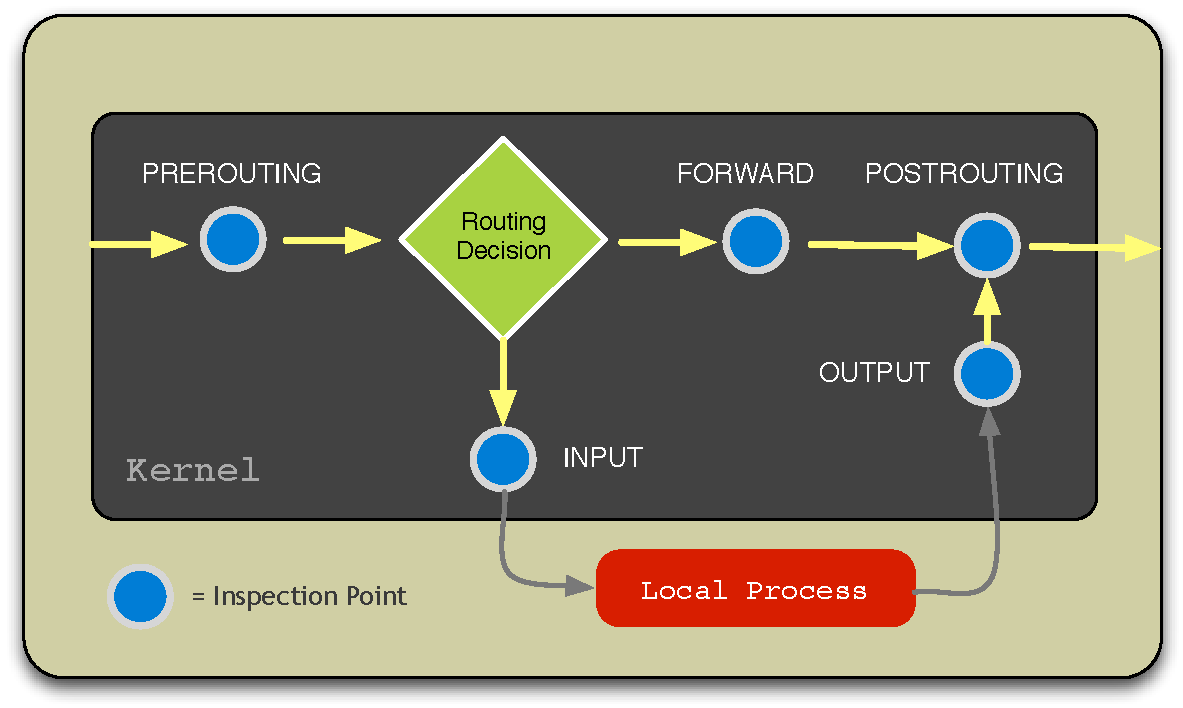
\includegraphics[scale=.6]{netfilter-packet-flow.pdf}
\end{frame} 

\begin{frame}{规则匹配}
\begin{itemize}
\item 规则排序列表
\item 包一次通过每一个规则的测试
\item 首次匹配,目标(target)开始工作:一般是退出链
\item 规则可以指定多个标准用来匹配
\item 规范里的每一个标准必须满足规则匹配
\item 如果没有匹配,则链策略应用
\end{itemize}

\end{frame} 
 \begin{frame}{简单例子}

filter表的一个 INPUT 规则

\medskip{}


\includegraphics[scale=.6]{iptables-demo.pdf}


\end{frame} 
 \begin{frame}{iptables结构}
\begin{itemize}
\item iptables将防火墙的功能分成多个tables

\begin{itemize}
\item filter:数据包过滤,\alert{默认是该功能,可以不用显示指定}
\item NAT:Network Address Translation/网络地址转换
\end{itemize}
\item tables又包含多个链(chain)

\begin{itemize}
\item 5条默认基础操作链
\item 允许用户自行定义链
\end{itemize}
\end{itemize}

\end{frame} 
 \begin{frame}[allowframebreaks]{iptables 语法}

iptables \emph{{[} -t table {]} <action> {[} pattern {]} {[} -j target
{]}}
\begin{itemize}
\item action包括

\begin{itemize}
\item -A chain: 在链中增加一条规则
\item -D chain: 在链中删除一条规则
\item -L chain: 列出链中的规则
\item -F chain: 清空链中的规则
\item -P chain: 为链指定新的默认策略,可以是:

\begin{itemize}
\item ACCEPT: 未经禁止,全部许可
\item DROP: 未经许可,全部禁止
\end{itemize}
\end{itemize}
\item pattern 包括

\begin{itemize}
\item -s <ip address>: 来源地址
\item -d <ip address>: 目标地址
\item -p <protocol>: 指定协议,可以是TCP/UDP/ICMP
\item --dport <port>: 目标端口,需要指定 -p
\item --sport <port>: 来源端口,需要指定 -p
\end{itemize}
\item 内建的 target 包括

\begin{itemize}
\item DROP:丢弃
\item ACCEPT:许可
\end{itemize}
\item 扩展的 target 包括

\begin{itemize}
\item LOG: 记录日志,关联到系统日志的kernel facility上,匹配LOG并不退出链
\item REJECT:拒绝,发一条提示给发送者
\item 定制链(chain)
\end{itemize}
\item Target 是可选的,但是一条规则上最多只有一个,如果没有,则应用缺省链策略
\end{itemize}

\end{frame} 
 \begin{frame}{基本链操作}


\begin{itemize}
\item -L/-vL 列出链或表的规则
\item -A 在链中追加一条规则
\item -I 在链中插入一条规则

\begin{itemize}
\item -I \emph{chain} (作为第一条规则插入)
\item -I \emph{chain 3} (作为规则3插入)
\end{itemize}
\item -D 删除一条独立的规则

\begin{itemize}
\item -D \emph{chain 3} 删除链中的规则3
\item -D \emph{chain rule} 显式的删除规则
\end{itemize}
\end{itemize}

\end{frame} 
 \begin{frame}{其他链操作}
\begin{itemize}
\item -P chain target 分配链策略,target有

\begin{description}
\item [{ACCEPT}] 内置,缺省设置
\item [{DROP}] 内置
\item [{REJECT}] 不允许,额外的 target
\end{description}
\item -F 清空一条链中的所有规则,但并不清空策略
\item -Z \emph{{[} chain {]} }包和字节计数器清零

\begin{itemize}
\item 用户监控链统计
\end{itemize}
\item -N,-X 管理定制的链

\begin{itemize}
\item -N your\_chain-name (增加链)
\item -X your\_chain-name (删除链)
\end{itemize}
\end{itemize}

\end{frame} 
 \begin{frame}{规则的一般考虑}
\begin{itemize}
\item 尽可能关闭

\begin{itemize}
\item iptables -P INPUT DROP 或
\item iptables -A INPUT -j DROP
\item iptables -A INPUT -j REJECT
\end{itemize}
\item 规则对回路同样适用

\begin{itemize}
\item 上面的简单例子对本地网络同样起到阻塞作用
\end{itemize}
\item 规则,就像路由一样,加载到内存里使用,必须保存到文件,才能在系统重启后还能生效
\end{itemize}

\end{frame} 
 \begin{frame}{匹配参数}
\begin{itemize}
\item 匹配可以由以下组成

\begin{itemize}
\item IP 地址或者主机名

\begin{itemize}
\item \alert{主机名是在规则插入时解析的}
\end{itemize}
\item 端口号,或者服务名
\item 参数可以用 ! 表示取反
\end{itemize}
\item 可以用'0:1023'来表示包括的端口范围
\item 子网掩码可以用VLSM或CIDR表示法
\end{itemize}

\end{frame} 

\begin{frame}[shrink]{惯用匹配标准}
\begin{itemize}
\item IP 地址或网络

\begin{itemize}
\item -s 192.168.0.0/24
\item -d 192.168.0.1
\end{itemize}
\item 网络接口

\begin{itemize}
\item -i lo
\item -o eth1
\end{itemize}
\item 用!取反

\begin{itemize}
\item -i eth0 -s ! 192.168.0.0/24
\end{itemize}
\item 传输协议和端口

\begin{itemize}
\item -p tcp --dport 80
\item -p udp --sport 53
\item 端口范围可以用 \emph{start:end} 指定
\end{itemize}
\item ICMP 类型

\begin{itemize}
\item -p icmp --icmp-type host-unreachable
\end{itemize}
\end{itemize}

\end{frame} 
 \begin{frame}{连接追踪}
\begin{itemize}
\item 提供包状态的检测,需要更多的内存
\item 使用'state'扩充匹配来实现
\item 可识别的状态有

\begin{description}
\item [{NEW}] 表示包已经开始一个新的连接,或者是和一个还没有在两端都有数据发送的连接关联
\item [{ESTABLISHED}] 表示包和一个两端都有数据发送的连接关联
\item [{RELATED}] 表示包正在建立一个新的连接,这个连接是和一个已建立的连接相关的,比如ftp data transfer,ICMP
error等
\item [{INVALID}] 表示这个包没有和已知的流或者连接与之关联,也可能是它包含的数据或者包头有问题
\end{description}
\end{itemize}

\end{frame} 
 \begin{frame}{链接追踪举例}
\begin{itemize}
\item 允许建立连接的规则\\
iptables -A INPUT -m state --state ESTABLISHED,RELATED - j ACCEPT
\item 多条规则,每一条对应一个服务的许可\\
iptables -A INPUT -m state --state NEW -p tcp --dport 25 -j ACCEPT
\item 最后,一个规则阻止所有其他入站请求\\
iptables -A INPUT -m state --state NEW -j DROP
\end{itemize}

\end{frame} 
 \begin{frame}{过滤表}


\begin{itemize}
\item 用于过滤数据包的传送
\item INPUT 链:

\begin{itemize}
\item 设定远端访问主机时的规则
\item 来源是远端访问者,目标是本地主机
\end{itemize}
\item OUTPUT 链:

\begin{itemize}
\item 设定主机访问远端主机的规则
\item 来源是本地主机,目标是远端被访问主机
\end{itemize}
\item FORWARD 链:

\begin{itemize}
\item 设定主机为其他主机转发数据包时的规则
\item 来源是请求转发的主机,目标是远端被访问的主机
\end{itemize}
\end{itemize}

\end{frame} 
 \begin{frame}{NAT 表}


\begin{itemize}
\item 将一个IP地址翻译成另外一个(入站或出站)
\item 允许多个内网IP地址“隐藏”在单个公网IP地址的后面
\item 使用 NAT 表设置规则
\item PREROUTING 链(DNAT):

\begin{itemize}
\item 路由算法发生之前
\item 转换数据包内的来源地址
\end{itemize}
\item POSTROUTING(SNAT,MASQUERADE) 链:

\begin{itemize}
\item 路由算法发生之后
\item 转换数据报内的目标地址
\end{itemize}
\end{itemize}

\end{frame} 
 \begin{frame}{SNAT例子}
\begin{itemize}
\item 对于负责内部子网的路由器,需要为保留地址进行IP伪装
\item 使用IP伪装功能需要打开本机上的IP转发功能
\item MASQUERADE\\
iptables –t nat –A POSTROUTING -s 192.168.0.0/24 -o eth1 –j MASQUERADE
\item SNAT\\
iptables -t nat -A POSTROUTING -j SNAT --to-source 220.220.220.220
\end{itemize}

\end{frame} 
 \begin{frame}{DNAT例子}
\begin{itemize}
\item 入站(INBOUND)\\
iptables -t nat -A PREROUTING -p tcp --dport 80 -j DNAT \textbackslash{}\\
--to-dest 192.168.1.20
\item 出站(OUTBOUND,带端口重定向)\\
iptables -t nat -A OUTPUT -p tcp --dport 80 -j DNAT \textbackslash{}\\
--to-dest 192.168.1.20:3128
\end{itemize}

\end{frame} 
 \begin{frame}{保存规则}
\begin{itemize}
\item iptables不是守护进程,它加载规则到内存,然后退出
\item service iptables save 可以保存当前的规则到/etc/sysconfig/iptables文件
\end{itemize}

\end{frame} 
 
\begin{frame}[fragile,plain]{/etc/sysconfig/iptables}
\begin{verbatim}
*filter 
:INPUT DROP [573:46163] 
:FORWARD ACCEPT [0:0] 
:OUTPUT ACCEPT [641:68532] 
-A INPUT -i lo -j ACCEPT 
-A INPUT -p tcp -m tcp –dport 143 -j ACCEPT 
-A INPUT -p tcp -m tcp –dport 22 -j ACCEPT 
-A INPUT -p tcp -m tcp –dport 25 -s 123.123.123.1 -j ACCEPT 
-A INPUT -p tcp -m tcp –dport 53 -j ACCEPT 
-A INPUT -p udp -m udp –dport 53 -j ACCEPT 
-A INPUT -p udp -m udp –dport 123 -s 123.123.123.1 -j ACCEPT 
-A INPUT -p icmp -j ACCEPT 
COMMIT
\end{verbatim}

\end{frame} 
 
% 
% \subsection{网络安全实验}
%
%
%
% \begin{frame}{实验I:用tcp\_wrappers限制服务}
%
%
%\begin{description}
%\item [{场景:}] 远程访问服务已经安装在你的系统上了。作为安全管理意识,你想控制这个访问,锁定系统,需要的时候才提供
%\item [{要求:}] 保护SSH和Telnet 服务
%\end{description}
%
%\end{frame} 
% \begin{frame}{实验II:对主机实现简单包过滤}
%
%
%\begin{description}
%\item [{场景:}] 你的部门已经选择部署防火墙到本地服务器上,需要执行简单的保护措施
%\item [{要求:}] 包过滤规则要求成功的限制连接到你的SSH和Telnet服务上
%\end{description}
%\end{frame}


% \section{数据安全}
%
%
%\end{frame} 
% \begin{frame}{数据安全}
%
%目标
%\begin{itemize}
%\item 理解基本的加密协议
%\item 描述Linux的加密实现
%\item 为常用网络协议配置加密服务
%\end{itemize}
%
%\end{frame} 
% \begin{frame}{需要加密}
%\begin{itemize}
%\item 非加密通信的危险倾向
%
%\begin{itemize}
%\item 密码/数据遭遇嗅探
%\item 操纵数据
%\item 操纵认证
%\item 等价于在明信片上邮件
%\end{itemize}
%\item 不安全的传统协议
%
%\begin{itemize}
%\item telnet,ftp,pop3,等:密码不安全
%\item sendmail,NFS,NIS,等:信息不安全
%\item rsh,rcp,等:认证不安全
%\end{itemize}
%\end{itemize}
%\end{frame} 
% \subsection{加密协议}
%
%
%
% \begin{frame}{加密方法}
%\begin{itemize}
%\item 随机数发生器
%\item 单项哈希(one way hashes)
%\item 对称算法
%\item 非对称(公钥)算法
%\item 公钥基础设施(PKI)
%\item 数字证书
%\item 实现
%
%\begin{itemize}
%\item openssl,gpg
%\end{itemize}
%\end{itemize}
%
%\end{frame} 
% \begin{frame}{随机数发生器}
%\begin{itemize}
%\item 伪随机数和熵源
%
%\begin{itemize}
%\item 键盘和鼠标事件
%\item 块设备中断
%\end{itemize}
%\item 内核提供熵源
%
%\begin{itemize}
%\item /dev/random
%
%\begin{itemize}
%\item 最好的源
%\item blocks when entropy pool exhausted
%\end{itemize}
%\item /dev/urandom
%
%\begin{itemize}
%\item 从熵池提取,知道耗尽
%\item 回退到伪随机数发生器
%\end{itemize}
%\end{itemize}
%\item openssl rand {[} -base64{]} \emph{num}
%\end{itemize}
%
%\end{frame} 
% \begin{frame}{单向哈希}
%\begin{itemize}
%\item 任意数据降低小“指纹”
%
%\begin{itemize}
%\item 任意长度输入
%\item 固定长度输入
%\item 如果数据改变,指纹也改变(“自由碰撞”)
%\item 数据不能从指纹重新产生(“单向”)
%\end{itemize}
%\item 惯用算法
%
%\begin{itemize}
%\item md2,md5,mdc2,rmd160,sha,sha1
%\end{itemize}
%\item 惯用工具
%
%\begin{itemize}
%\item sha1sum {[} --check {]} \emph{file}
%\item md5sum {[} --check {]} \emph{file}
%\item openssl,gpg
%\item rpm -V
%\end{itemize}
%\end{itemize}
%
%\end{frame} 
% \begin{frame}{对称加密}
%\begin{itemize}
%\item 基于单键
%
%\begin{itemize}
%\item 同时用于加密和解密
%\end{itemize}
%\item 常用算法
%
%\begin{itemize}
%\item DES,3DES,Blowfish,RC2,RC4,RC5,IDEA,CAST5
%\end{itemize}
%\item 实用工具
%
%\begin{itemize}
%\item passwd (修改DES)
%\item gpg(3DES,CAST5,Blowfish)
%\item openssl
%\end{itemize}
%\end{itemize}
%
%\end{frame} 
% \begin{frame}{[allowframebreaks]非对称加密}
%\begin{itemize}
%\item 基于公/私钥对
%
%\begin{itemize}
%\item 一把用来加密,另外一把解密
%\end{itemize}
%\item 协议 I:无键同步加密
%
%\begin{itemize}
%\item 收信人
%
%\begin{itemize}
%\item 生成公/私钥对:P和S
%\item 发布公钥P,保管私钥S
%\end{itemize}
%\item 发信人
%
%\begin{itemize}
%\item 用公钥加密消息M
%\item 发送P(M)给收信人
%\end{itemize}
%\item 收信人
%
%\begin{itemize}
%\item 用私钥解密:M=S(P(M))
%\end{itemize}
%\end{itemize}
%\item 协议 II :数字签名
%
%\begin{itemize}
%\item 发信人
%
%\begin{itemize}
%\item 生成公/私钥对:P和S
%\item 发布公钥P,保管私钥S
%\item 用私钥S加密消息M
%\item 发给收信人S(M)
%\end{itemize}
%\item 收信人
%
%\begin{itemize}
%\item 用发信人发给的公钥揭秘恢复 M=P(S(M))
%\end{itemize}
%\end{itemize}
%\item 结合签名和加密
%\item 签名分离
%\end{itemize}
%
%\end{frame} 
% \begin{frame}{公钥基础设施(PKI)}
%\begin{itemize}
%\item 非对称加密依赖公钥的一致性
%\item 两个方法阻止公钥欺骗
%
%\begin{itemize}
%\item 发布密钥指纹
%\item 公钥基础设施(PKI)
%
%\begin{itemize}
%\item 由信任的站点分发
%\item 分层的认证中心(CA)-- 数字证书
%\end{itemize}
%\end{itemize}
%\end{itemize}
%
%\end{frame} 
% \begin{frame}{数字证书}
%\begin{itemize}
%\item 认证中心(Certificate Authorities,CA)
%\item 数字证书
%
%\begin{itemize}
%\item 所有人:Public Key和Identity
%\item 发行人:分离的签名和Identity
%\item 有效周期
%\end{itemize}
%\item 类型
%
%\begin{itemize}
%\item 认证中心证书
%\item 服务器证书
%\end{itemize}
%\item 自签名证书
%\end{itemize}
%
%\end{frame} 
% \begin{frame}{生成数字证书}
%\begin{itemize}
%\item X.509证书格式
%\item 生成公/私钥对,定义身份
%\item 两个选项
%
%\begin{itemize}
%\item 使用CA
%
%\begin{itemize}
%\item 生成签名申请(csr)
%\item 发送csr到CA
%\item 从CA收到签名
%\end{itemize}
%\item 自签名证书
%
%\begin{itemize}
%\item 用自己的公钥签名
%\end{itemize}
%\end{itemize}
%\end{itemize}
%\end{frame}


